\documentclass{standalone}
\usepackage{tikz}

\begin{document}

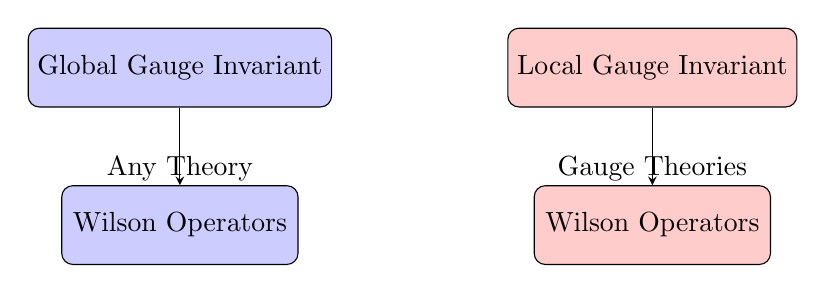
\begin{tikzpicture}[node distance=2cm]

% Define styles for nodes
\tikzset{
    operator/.style={draw, rectangle, rounded corners, minimum width=3cm, minimum height=1cm},
    global/.style={fill=blue!20},
    local/.style={fill=red!20}
}

% Nodes for global gauge invariant Wilson operators
\node[operator, global] (global1) {Global Gauge Invariant};
\node[operator, global, below of=global1] (global2) {Wilson Operators};

% Nodes for local gauge invariant Wilson operators
\node[operator, local, right of=global1, xshift=4cm] (local1) {Local Gauge Invariant};
\node[operator, local, below of=local1] (local2) {Wilson Operators};

% Arrows connecting the categories
\draw[-stealth] (global1.south) -- node[below] {Any Theory} (global2.north);
\draw[-stealth] (local1.south) -- node[below] {Gauge Theories} (local2.north);

\end{tikzpicture}

\end{document}